
%%%%%%%%%%%%%%%%%%%%%%%%%%%%%%%%%%%%%%%%%%%%%%%%%%%%%%%%%
%%% 对称配筋柱正截面计算题例1
%%%%%%%%%%%%%%%%%%%%%%%%%%%%%%%%%%%%%%%%%%%%%%%%%%%%%%%%%

\begin{frame}[plain]{ 对称配筋柱正截面计算题例1 }
\begin{columns}[onlytextwidth]
\begin{column}{0.75\textwidth}
偏心受压柱,已知:\\
柱计算高度:$l_c= 3.5 m$ 。 \\
矩形截面:$b \times h = 300 \times 400 mm^2$。\\
材料:采用纵筋~HRB400,C30 混凝土。\\
内力:$(M_t, M_b, N) = ( -200 kN\cdot m, 70 kN\cdot m, 750 kN)$ \\
按对称配筋柱计算所需纵筋(取$a_s = 40 mm, a'_s = 40 mm$)。\\
\end{column}

\begin{column}{0.25\textwidth}
\begin{center}
\scalebox{0.5}{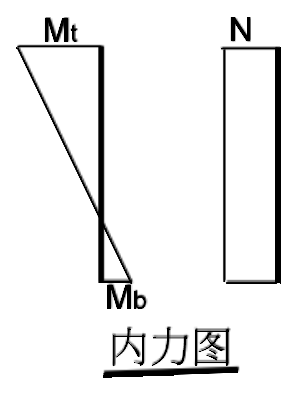
\includegraphics{fig1.eps}}
\end{center}
\end{column}

\end{columns}
\end{frame}

\begin{frame}[plain]
解:一、二阶效应的计算
\vspace{-0.5em}
\begin{align*}
	& h_0 = h - a_s = 400 - 40 = 360 mm &\\ 
	\uncover<2-> {& M_2 = max(|M_t|, |M_b|)= 200 kN\cdot m &\\ 
	& M_1 = \frac{M_t\cdot M_b}{|M_t|\cdot|M_b|}min(|M_t|, |M_b|)= -70 kN\cdot m  &\\}
	\uncover<3-> {& \frac{M_1} {M_2} = \frac{ -70 } { 200 } = -0.350 } &\\
	\uncover<4-> {& i = h/\sqrt{12} = 400 / \sqrt{12} = 115.5 mm  &\\}
	\uncover<5-> {& \frac{l_c} {i} = \frac{ 3.5\times10^3 } { 115.5 } =    30.3 &\\ }
	\uncover<6-> {& \frac{N}{f_cA} = \frac{ 750\times10^3 }{ 14.3\times 300\times 400 } =  0.437&}
\end{align*}
\end{frame}

%%% M_1/M_2 > 0.9
%%%
%%%
\begin{frame}[plain]
\vspace{-0.5em}
因为
\begin{align*}
	\uncover<2-> {(1)\quad & \frac{l_c} {i} =   30.3 <  &\\ 
			&34 - 12(M_1/M_2) = 34 - 12 \times   -0.3 =   38.2 &\\} 
	\uncover<3-> {(2)\quad & \frac{M_1}{M_2}= -0.350 < 0.9 &\\}
	\uncover<4-> {(3)\quad & \frac{N}{f_c A} =  0.437 < 0.9 &\\}
\end{align*} 
\uncover<5-> {所以:不用考虑二阶效应,取 $M = M_2 = 200kN\cdot m $}
\end{frame}
%%%

\begin{frame}[plain]
二、偏心距的计算 
\beamerdefaultoverlayspecification{<+-}
\begin{align*}
	& e_0 = \frac{M} {N} = \frac{ 200 } { 750} m = 267 mm &\\
	\uncover<2->{& e_a = max(20, 400/30) =  20mm  &\\ }
	\uncover<3->{& e_i = e_0 + e_a = 267 +  20 =  287 mm &\\ }  
	\uncover<4->{& e = e_i + 0.5h - a_s &\\ 
		     &\mspace{9mu} =  287 + 0.5 \times 400 - 40 =    447 mm &\\}  
	\uncover<5->{& e' = e_i - 0.5h + a'_s &\\ 
		     &\mspace{9mu} =  287 - 0.5 \times 400 + 40 =    127 mm &\\}  
\end{align*} 
\end{frame}

\begin{frame}[plain]
三、假设为受拉破坏
\begin{align*}
	& x = \frac{N} {\alpha_1 f_c b} = \frac{ 750\times 10^3} {1.0 \times 14.3 \times 300 } =  174.8 mm &
\end{align*}
%%% 
\begin{align*}
	\uncover<2-> { & > 2a'_s = 2\times 40 = 80.0 mm &\\ 
		       & < \xi_b \times h_0 = 0.518 \times 360 =  186.5 mm &\\ } 
	\uncover<3-> { & \text{假设正确,且受压纵筋能屈服。} &\\ 
	     	& A_s = A'_s = \frac{Ne - \alpha_1 f_c b x (h_0 - 0.5x)}{f\mspace{3mu}'_y(h_0 - a'_s)} \mspace{10mu}&\\ 
		& = \frac{ 750 \times 10^3 \times    447 - 1.0 \times 14.3 \times 300 
		\times  174.8 \times (360 - 0.5 \times  174.8 )} 
		{ 360 \times (360 - 40.0) } &\\
	    	& \mspace{10mu} = 1133.3 mm^2 &\\ }
\end{align*}
%%%
%%%
%%% 配筋率验算
\begin{align*} 
%%%	
	\uncover<4-> { & > 0.2\% \times 300 \times 400 =  240.0 mm^2 \text{,单侧配筋率满足要求}&\\ }
%%%
%%%
%%%
	\uncover<5-> { & A_s+A'_s > 0.55\% \times 300 \times 400 
	=  660.0 mm^2 \text{,双侧配筋率满足要求}&\\ }
%%%
\end{align*}
\end{frame}



%%%%%%%%%%%%%%%%%%%%%%%%%%%%%%%%%%%%%%%%%%%%%%%%%%%%%%%%%
%%% 对称配筋柱正截面计算题2
%%%%%%%%%%%%%%%%%%%%%%%%%%%%%%%%%%%%%%%%%%%%%%%%%%%%%%%%%

\begin{frame}[plain]{ 对称配筋柱正截面计算题2 }
\begin{columns}[onlytextwidth]
\begin{column}{0.75\textwidth}
偏心受压柱,已知:\\
柱计算高度:$l_c= 4.5 m$ 。 \\
矩形截面:$b \times h = 300 \times 400 mm^2$。\\
材料:采用纵筋~HRB400,C30 混凝土。\\
内力:$(M_t, M_b, N) = ( -200 kN\cdot m, 70 kN\cdot m, 750 kN)$ \\
按对称配筋柱计算所需纵筋(取$a_s = 40 mm, a'_s = 40 mm$)。\\
\end{column}

\begin{column}{0.25\textwidth}
\begin{center}
\scalebox{0.5}{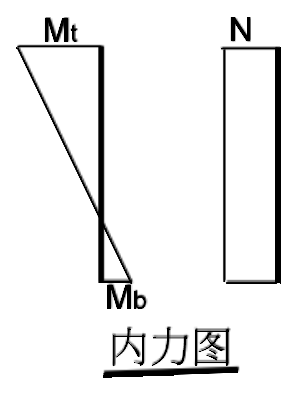
\includegraphics{fig1.eps}}
\end{center}
\end{column}

\end{columns}
\end{frame}

\begin{frame}[plain]
解:一、二阶效应的计算
\vspace{-0.5em}
\begin{align*}
	& h_0 = h - a_s = 400 - 40 = 360 mm &\\ 
	\uncover<2-> {& M_2 = max(|M_t|, |M_b|)= 200 kN\cdot m &\\ 
	& M_1 = \frac{M_t\cdot M_b}{|M_t|\cdot|M_b|}min(|M_t|, |M_b|)= -70 kN\cdot m  &\\}
	\uncover<3-> {& \frac{M_1} {M_2} = \frac{ -70 } { 200 } = -0.350 } &\\
	\uncover<4-> {& i = h/\sqrt{12} = 400 / \sqrt{12} = 115.5 mm  &\\}
	\uncover<5-> {& \frac{l_c} {i} = \frac{ 4.5\times10^3 } { 115.5 } =    39.0 &\\ }
	\uncover<6-> {& \frac{N}{f_cA} = \frac{ 750\times10^3 }{ 14.3\times 300\times 400 } =  0.437&}
\end{align*}
\end{frame}

%%% M_1/M_2 > 0.9
%%%
%%%
\begin{frame}[plain]
因为
\begin{align*}
	\uncover<2-> {&
	\frac{l_c} {i} =   39.0 >  34 - 12(M_1/M_2) = 34 - 12 \times   -0.3 
	=   38.2 &} 
\end{align*}
\uncover<3-> {所以:要考虑附加弯矩\\}
\vspace{-1.5em}
\begin{align*}
	\uncover<4-> {&C_m = max(0.7, 0.7+0.3M_1/M_2) &\\ 
	\mspace{9mu} &= max(0.7, 0.7+0.3\times-70 / 200 )=0.700 &\\}
	\uncover<5->{& e_a = max(20, 400/30) =  20mm  &\\ }
	\uncover<6->{& \zeta_c = min(1.0, \frac{0.5f_cA}{N}) = min(1.0, 0.5\times 0.437)=0.219 &\\ }
\end{align*}
\end{frame}

\begin{frame}[plain]
\vspace{-0.5em}
\begin{align*}
	\uncover<2->{& \eta_{ns} = 1+ \frac{1}{1300(M_2/N + e_a)/h_0}(\frac{l_c}{h})^2 \zeta_c &\\}
	\uncover<3->{& \mspace{9mu} = 1+\frac{ 360 }{1300( 200/750\times 10^3+   20)}
					(\frac{ 4.5\times10^3 }{ 400 } )^2\times 0.219 &\\
	&= 1.027 &\\}
	\uncover<4->{& M = max(1.0, C_m \eta_{ns}) &\\
		     & \mspace{10mu}= max(1.0, 0.700\times 1.027)\times 200 &\\
		&=  200.0 &\\}
\end{align*}
\end{frame}

%%%
%%%

\begin{frame}[plain]
二、偏心距的计算 
\beamerdefaultoverlayspecification{<+-}
\begin{align*}
	& e_0 = \frac{M} {N} = \frac{ 200 } { 750} m = 267 mm &\\
	\uncover<2->{& e_a = max(20, 400/30) =  20mm  &\\ }
	\uncover<3->{& e_i = e_0 + e_a = 267 +  20 =  287 mm &\\ }  
	\uncover<4->{& e = e_i + 0.5h - a_s &\\ 
		     &\mspace{9mu} =  287 + 0.5 \times 400 - 40 =    447 mm &\\}  
	\uncover<5->{& e' = e_i - 0.5h + a'_s &\\ 
		     &\mspace{9mu} =  287 - 0.5 \times 400 + 40 =    127 mm &\\}  
\end{align*} 
\end{frame}

\begin{frame}[plain]
三、假设为受拉破坏
\begin{align*}
	& x = \frac{N} {\alpha_1 f_c b} = \frac{ 750\times 10^3} {1.0 \times 14.3 \times 300 } =  174.8 mm &
\end{align*}
%%% 
\begin{align*}
	\uncover<2-> { & > 2a'_s = 2\times 40 = 80.0 mm &\\ 
		       & < \xi_b \times h_0 = 0.518 \times 360 =  186.5 mm &\\ } 
	\uncover<3-> { & \text{假设正确,且受压纵筋能屈服。} &\\ 
	     	& A_s = A'_s = \frac{Ne - \alpha_1 f_c b x (h_0 - 0.5x)}{f\mspace{3mu}'_y(h_0 - a'_s)} \mspace{10mu}&\\ 
		& = \frac{ 750 \times 10^3 \times    447 - 1.0 \times 14.3 \times 300 
		\times  174.8 \times (360 - 0.5 \times  174.8 )} 
		{ 360 \times (360 - 40.0) } &\\
	    	& \mspace{10mu} = 1133.3 mm^2 &\\ }
\end{align*}
%%%
%%%
%%% 配筋率验算
\begin{align*} 
%%%	
	\uncover<4-> { & > 0.2\% \times 300 \times 400 =  240.0 mm^2 \text{,单侧配筋率满足要求}&\\ }
%%%
%%%
%%%
	\uncover<5-> { & A_s+A'_s > 0.55\% \times 300 \times 400 
	=  660.0 mm^2 \text{,双侧配筋率满足要求}&\\ }
%%%
\end{align*}
\end{frame}



%%%%%%%%%%%%%%%%%%%%%%%%%%%%%%%%%%%%%%%%%%%%%%%%%%%%%%%%%
%%% 对称配筋柱正截面计算题3
%%%%%%%%%%%%%%%%%%%%%%%%%%%%%%%%%%%%%%%%%%%%%%%%%%%%%%%%%

\begin{frame}[plain]{ 对称配筋柱正截面计算题3 }
\begin{columns}[onlytextwidth]
\begin{column}{0.75\textwidth}
偏心受压柱,已知:\\
柱计算高度:$l_c= 3.5 m$ 。 \\
矩形截面:$b \times h = 300 \times 400 mm^2$。\\
材料:采用纵筋~HRB400,C30 混凝土。\\
内力:$(M_t, M_b, N) = ( 200 kN\cdot m, -70 kN\cdot m, 250 kN)$ \\
按对称配筋柱计算所需纵筋(取$a_s = 40 mm, a'_s = 40 mm$)。\\
\end{column}

\begin{column}{0.25\textwidth}
\begin{center}
\scalebox{0.5}{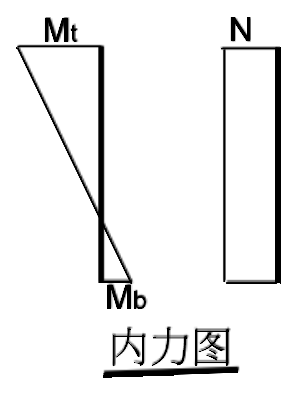
\includegraphics{fig1.eps}}
\end{center}
\end{column}

\end{columns}
\end{frame}

\begin{frame}[plain]
解:一、二阶效应的计算
\vspace{-0.5em}
\begin{align*}
	& h_0 = h - a_s = 400 - 40 = 360 mm &\\ 
	\uncover<2-> {& M_2 = max(|M_t|, |M_b|)= 200 kN\cdot m &\\ 
	& M_1 = \frac{M_t\cdot M_b}{|M_t|\cdot|M_b|}min(|M_t|, |M_b|)= -70 kN\cdot m  &\\}
	\uncover<3-> {& \frac{M_1} {M_2} = \frac{ -70 } { 200 } = -0.350 } &\\
	\uncover<4-> {& i = h/\sqrt{12} = 400 / \sqrt{12} = 115.5 mm  &\\}
	\uncover<5-> {& \frac{l_c} {i} = \frac{ 3.5\times10^3 } { 115.5 } =    30.3 &\\ }
	\uncover<6-> {& \frac{N}{f_cA} = \frac{ 250\times10^3 }{ 14.3\times 300\times 400 } =  0.146&}
\end{align*}
\end{frame}

%%% M_1/M_2 > 0.9
%%%
%%%
\begin{frame}[plain]
\vspace{-0.5em}
因为
\begin{align*}
	\uncover<2-> {(1)\quad & \frac{l_c} {i} =   30.3 <  &\\ 
			&34 - 12(M_1/M_2) = 34 - 12 \times   -0.3 =   38.2 &\\} 
	\uncover<3-> {(2)\quad & \frac{M_1}{M_2}= -0.350 < 0.9 &\\}
	\uncover<4-> {(3)\quad & \frac{N}{f_c A} =  0.146 < 0.9 &\\}
\end{align*} 
\uncover<5-> {所以:不用考虑二阶效应,取 $M = M_2 = 200kN\cdot m $}
\end{frame}
%%%

\begin{frame}[plain]
二、偏心距的计算 
\beamerdefaultoverlayspecification{<+-}
\begin{align*}
	& e_0 = \frac{M} {N} = \frac{ 200 } { 250} m = 800 mm &\\
	\uncover<2->{& e_a = max(20, 400/30) =  20mm  &\\ }
	\uncover<3->{& e_i = e_0 + e_a = 800 +  20 =  820 mm &\\ }  
	\uncover<4->{& e = e_i + 0.5h - a_s &\\ 
		     &\mspace{9mu} =  820 + 0.5 \times 400 - 40 =    980 mm &\\}  
	\uncover<5->{& e' = e_i - 0.5h + a'_s &\\ 
		     &\mspace{9mu} =  820 - 0.5 \times 400 + 40 =    660 mm &\\}  
\end{align*} 
\end{frame}

\begin{frame}[plain]
三、假设为受拉破坏
\begin{align*}
	& x = \frac{N} {\alpha_1 f_c b} = \frac{ 250\times 10^3} {1.0 \times 14.3 \times 300 } =   58.3 mm &
\end{align*}
%%%
%%% 受压纵筋不屈服
\begin{align*}
	\uncover<2-> { & < 2a'_s = 2\times 40 = 80.0 mm &\\ }
	\uncover<3-> { & \text{假设正确,但受压纵筋不屈服。} &\\ 
		& A_s = A'_s = \frac{Ne'}{f\mspace{3mu}'_y(h_0 - a'_s)}\mspace{10mu} &\\ 
	       	& = \frac{ 250 \times 10^3 \times    660 }{ 360\times (360 - 40.0 )} &\\
	       	&\mspace{10mu} = 1432.3 }
\end{align*}
%%%%
%%%
%%%
%%% 配筋率验算
\begin{align*} 
%%%	
	\uncover<4-> { & > 0.2\% \times 300 \times 400 =  240.0 mm^2 \text{,单侧配筋率满足要求}&\\ }
%%%
%%%
%%%
	\uncover<5-> { & A_s+A'_s > 0.55\% \times 300 \times 400 
	=  660.0 mm^2 \text{,双侧配筋率满足要求}&\\ }
%%%
\end{align*}
\end{frame}



%%%%%%%%%%%%%%%%%%%%%%%%%%%%%%%%%%%%%%%%%%%%%%%%%%%%%%%%%
%%% 对称配筋柱计算题4
%%%%%%%%%%%%%%%%%%%%%%%%%%%%%%%%%%%%%%%%%%%%%%%%%%%%%%%%%

\begin{frame}[plain]{ 对称配筋柱计算题4 }
\begin{columns}[onlytextwidth]
\begin{column}{0.75\textwidth}
偏心受压柱,已知:\\
柱计算高度:$l_c= 3.5 m$ 。 \\
矩形截面:$b \times h = 300 \times 400 mm^2$。\\
材料:采用纵筋~HRB400,C30 混凝土。\\
内力:$(M_t, M_b, N) = ( 200 kN\cdot m, -70 kN\cdot m, 2500 kN)$ \\
按对称配筋柱计算所需纵筋(取$a_s = 40 mm, a'_s = 40 mm$)。\\
\end{column}

\begin{column}{0.25\textwidth}
\begin{center}
\scalebox{0.5}{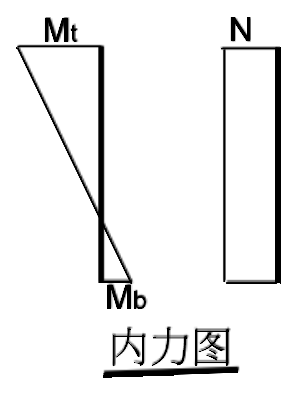
\includegraphics{fig1.eps}}
\end{center}
\end{column}

\end{columns}
\end{frame}

\begin{frame}[plain]
解:一、二阶效应的计算
\vspace{-0.5em}
\begin{align*}
	& h_0 = h - a_s = 400 - 40 = 360 mm &\\ 
	\uncover<2-> {& M_2 = max(|M_t|, |M_b|)= 200 kN\cdot m &\\ 
	& M_1 = \frac{M_t\cdot M_b}{|M_t|\cdot|M_b|}min(|M_t|, |M_b|)= -70 kN\cdot m  &\\}
	\uncover<3-> {& \frac{M_1} {M_2} = \frac{ -70 } { 200 } = -0.350 } &\\
	\uncover<4-> {& i = h/\sqrt{12} = 400 / \sqrt{12} = 115.5 mm  &\\}
	\uncover<5-> {& \frac{l_c} {i} = \frac{ 3.5\times10^3 } { 115.5 } =    30.3 &\\ }
	\uncover<6-> {& \frac{N}{f_cA} = \frac{ 2500\times10^3 }{ 14.3\times 300\times 400 } =  1.457&}
\end{align*}
\end{frame}

%%% M_1/M_2 > 0.9
%%%
%%%
\begin{frame}[plain]
\vspace{-0.5em}
\begin{align*}
	\uncover<2-> {&\text{因为}  \frac{N}{f_c A} =  1.457 > 0.9 &\\}
\end{align*}
\uncover<3-> {所以:要考虑附加弯矩\\}
\vspace{-1.5em}
\begin{align*}
	\uncover<4-> {&C_m = max(0.7, 0.7+0.3M_1/M_2) &\\ 
	\mspace{9mu} &= max(0.7, 0.7+0.3\times-70 / 200 )=0.700 &\\}
	\uncover<5->{& e_a = max(20, 400/30) =  20mm  &\\ }
	\uncover<6->{& \zeta_c = min(1.0, \frac{0.5f_cA}{N}) 
			= min(1.0, 0.5\times 1.457)=0.728 &\\ }
\end{align*}
\end{frame}

%%%%%%%
\begin{frame}[plain]
\vspace{-0.5em}
\begin{align*}
	\uncover<2->{& \eta_{ns} = 1+ \frac{1}{1300(M_2/N + e_a)/h_0}(\frac{l_c}{h})^2 \zeta_c &\\}
	\uncover<3->{& \mspace{9mu} = 1+\frac{ 360 }{1300( 200/2500\times 10^3+   20)}
						(\frac{ 3.5\times10^3 }{ 400 } )^2\times 0.728 &\\
		     &= 1.154 &\\}
	\uncover<4->{& M = max(1.0, C_m \eta_{ns}) &\\
		     & \mspace{10mu}= max(1.0, 0.700\times 1.154)\times 200 &\\
		     &=  200.0 &\\}
\end{align*}
\end{frame}
%%%
%%%

\begin{frame}[plain]
二、偏心距的计算 
\beamerdefaultoverlayspecification{<+-}
\begin{align*}
	& e_0 = \frac{M} {N} = \frac{ 200 } { 2500} m =  80 mm &\\
	\uncover<2->{& e_a = max(20, 400/30) =  20mm  &\\ }
	\uncover<3->{& e_i = e_0 + e_a =  80 +  20 =  100 mm &\\ }  
	\uncover<4->{& e = e_i + 0.5h - a_s &\\ 
		     &\mspace{9mu} =  100 + 0.5 \times 400 - 40 =    260 mm &\\}  
	\uncover<5->{& e' = e_i - 0.5h + a'_s &\\ 
		     &\mspace{9mu} =  100 - 0.5 \times 400 + 40 =     60 mm &\\}  
\end{align*} 
\end{frame}

\begin{frame}[plain]
三、假设为受拉破坏
\begin{align*}
	& x = \frac{N} {\alpha_1 f_c b} = \frac{ 2500\times 10^3} {1.0 \times 14.3 \times 300 } =  582.8 mm &
\end{align*}
%%%
%%% 受拉纵筋不屈服
\begin{align*}
	\uncover<2->{ &x > \xi_b h_0 = 0.518\times360=186.5, \text{假设错误,按受压破坏计算} &\\}
	\uncover<3->{ &\xi = \frac{%%frac first part
				N-\xi_b\alpha_1 f_c bh_0}{\frac{Ne - 0.43\alpha_1 f_c bh^2_0
			}{%%frac second part
				(\beta_1 - \xi_b)(h_0 - a'_s)
			}%%end frac
			+ \alpha_1 f_c bh_0} + \xi_b &\\ 
		      &\mspace{10mu}= \frac{%%frac first
				2500\times10^3 - 0.518\times1.0\times14.3\times300\times360~
			}{%%frac second
				\frac{%%%frac first
					2500\times10^3\times260-0.43\times1.0\times14.3\times300\times360^2~
				}{%%%frac second
					(0.8-0.518)(360-40)~
				}
				+ 1.0\times14.3\times300\times360~
			} &\\
			 &\mspace{14mu}+  0.518 =  0.797 &\\
		}
	\uncover<4->{&A_s=A'_s = \frac{%%frac first
				Ne - \alpha_1 f_c bh^2_0 \xi(1-0.5\xi)
			}{%%frac seconcd
				f'_y(h_0 - a'_s)	
			} &\\
		  &\mspace{10mu}\frac{%%frac first
				2500(10^3)\times 260 - 1.0\times14.3\times300\times360^2\times0.797(1-0.5\times0.797)
			}{%%frac seconc
				360\times(360 - 40)
			} &\\
		   &\mspace{10mu} =  3328.9 mm^2 \text{配筋率验算略}	&
		}		
\end{align*}
%%%
%%%
%%%
%%% 配筋率验算
\begin{align*} 
%%%	
	\uncover<4-> { & > 0.2\% \times 300 \times 400 =  240.0 mm^2 \text{,单侧配筋率满足要求}&\\ }
%%%
%%%
%%%
	\uncover<5-> { & A_s+A'_s > 0.55\% \times 300 \times 400 
	=  660.0 mm^2 \text{,双侧配筋率满足要求}&\\ }
%%%
\end{align*}
\end{frame}


